\documentclass[10pt]{article}
\usepackage[polish]{babel}
\usepackage[utf8]{inputenc}
\usepackage[T1]{fontenc}
\usepackage{amsmath}
\usepackage{amsfonts}
\usepackage{amssymb}
\usepackage[version=4]{mhchem}
\usepackage{stmaryrd}
\usepackage{graphicx}
\usepackage[export]{adjustbox}
\graphicspath{ {./images/} }

\title{LIGA MATEMATYCZNA im. Zdzisława Matuskiego \\
 FINAE \\
 24 kwietnia 2017 SZKOŁA PODSTAWOWA }

\author{}
\date{}


\begin{document}
\maketitle
\section*{ZADANIE 1.}
Ania miała 96 jednakowych patyczków i zbudowała z nich kwadraty i trójkąty. Boki wszystkich figur miały długość jednego patyczka. Powstało 27 rozłącznych figur przy wykorzystaniu wszystkich patyczków. Ile kwadratów i ile trójkątów zbudowała Ania?

\section*{ZADANIE 2.}
Wszystkie figury znajdujące się wewnątrz prostokąta są kwadratami. Czarny kwadrat ma pole 1, kwadrat \(A\) ma pole 81 . Wyznacz pole kwadratu \(X\) oraz oblicz obwód dużego prostokąta.\\
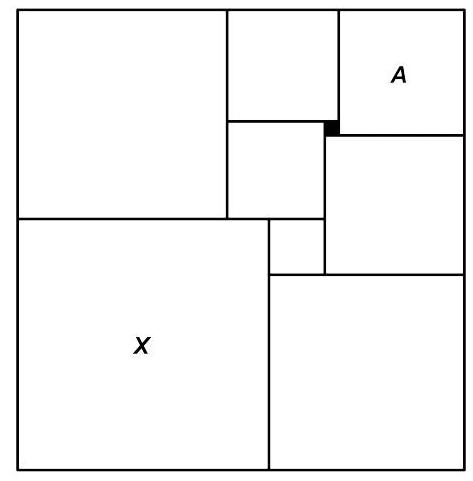
\includegraphics[max width=\textwidth, center]{2024_11_21_14af575c41c1c56d2472g-1}

\section*{ZADANIE 3.}
Ania i Bartek odrabiają pracę domową. Ania ma znaleźć najmniejszą liczbę naturalną podzielną przez sześć kolejnych liczb nieparzystych, a Bartek - najmniejszą liczbę naturalną podzielną przez osiem kolejnych liczb parzystych. Czyja liczba będzie mniejsza?

\section*{ZADANIE 4.}
W pewnej rodzinie jest pięć córek: Ania, Basia, Czesia, Daria i Ela. Rodziły się one w podanej kolejności co trzy lata. Najstarsza Ania jest siedem razy starsza od najmłodszej Eli. Ile lat ma Czesia?

\section*{ZADANIE 5.}
Przez jaką liczbę należy podzielić liczby 331 i 459, aby w obu przypadkach otrzymać resztę z dzielenia równą 11? Podaj wszystkie rozwiązania.


\end{document}